\section{Evaluation}
\label{sec:evaluation}

Here we perform two experiments to quantify the performance of the S3 RAID-6 system and draw several conclusions based on our results.

First we experimentally determine the time required to distribute a file in the S3-RAID-6 array.
We call this the file store duration.
We estimate file store duration for a range of file sizes and report our results in Fig.\ref{fig:S3R6Str}.

Next we run an experiment to estimate the recover time of the system from failures.
Our experiment methods is as follows.
First, we store a file of known size in the S3-RAID6 array.
Second, we chose $M$ number of random disks and delete them.
Thirdly, we start the timer and estimate the recovery duration.
During the recovery process, data from all buckets (disks) are downloaded by the RAID controller. 
It then checks for missing disks, reconstructs the lost data and re-uploads the same.
The timer is stopped after a successful re-upload.
We repeat this process for a range of file sizes and report our results in Fig.\ref{fig:S3R6Rcv}.
As expected, our results suggest that the performance of our system is strongly correlated with network speed.

\begin{figure}[h!]
\centering
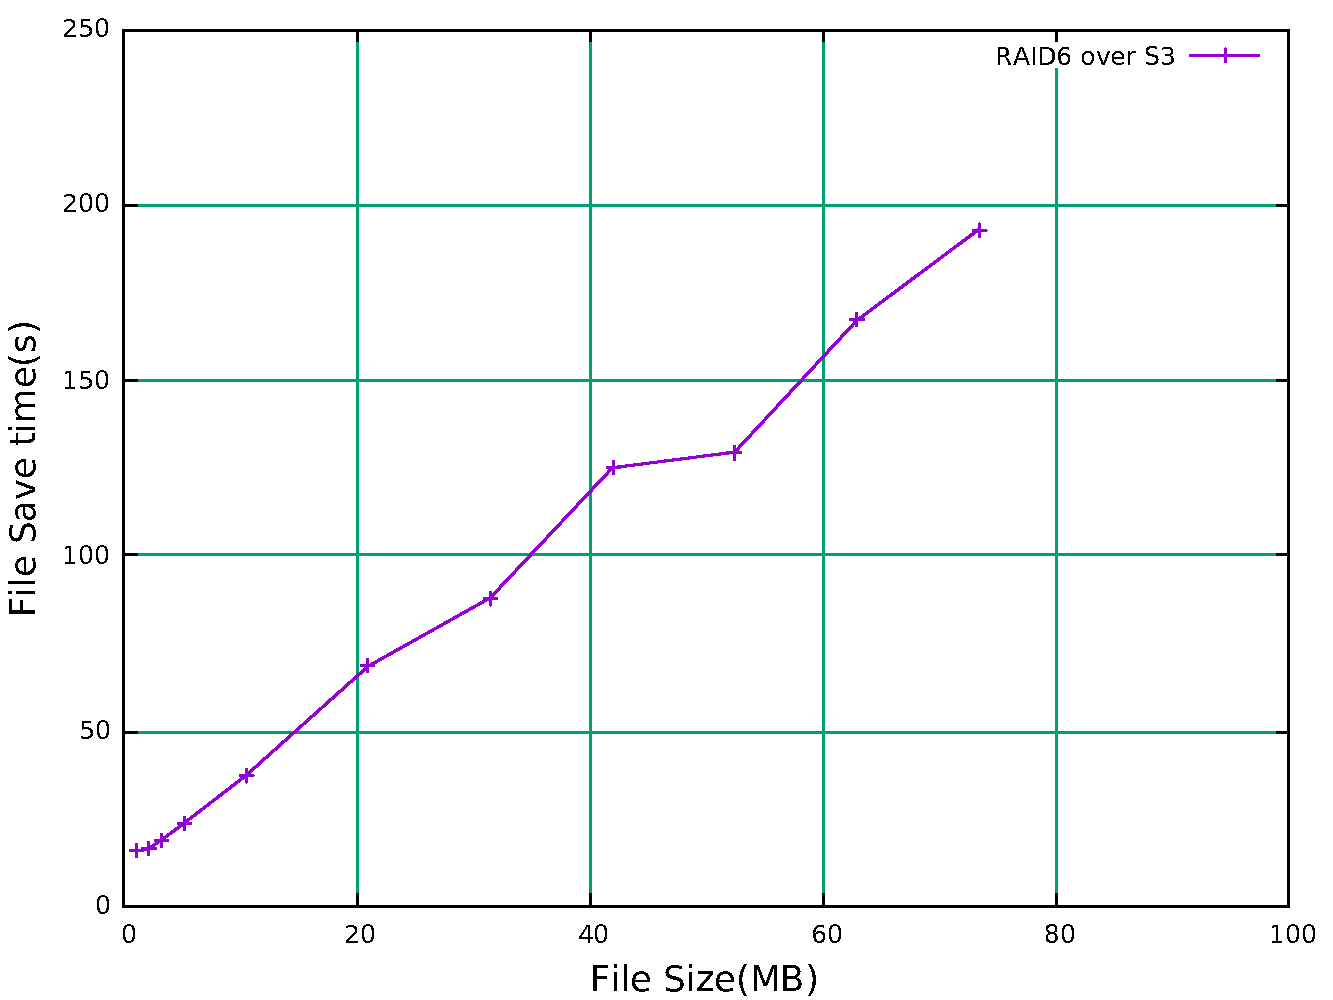
\includegraphics[width=\linewidth]{figures/S3RAIDStoreTime.pdf}
\caption{Time duration in seconds to store a file in S3 for varying file sizes.}
\label{fig:S3R6Str}
\end{figure}

\begin{figure}[h!]
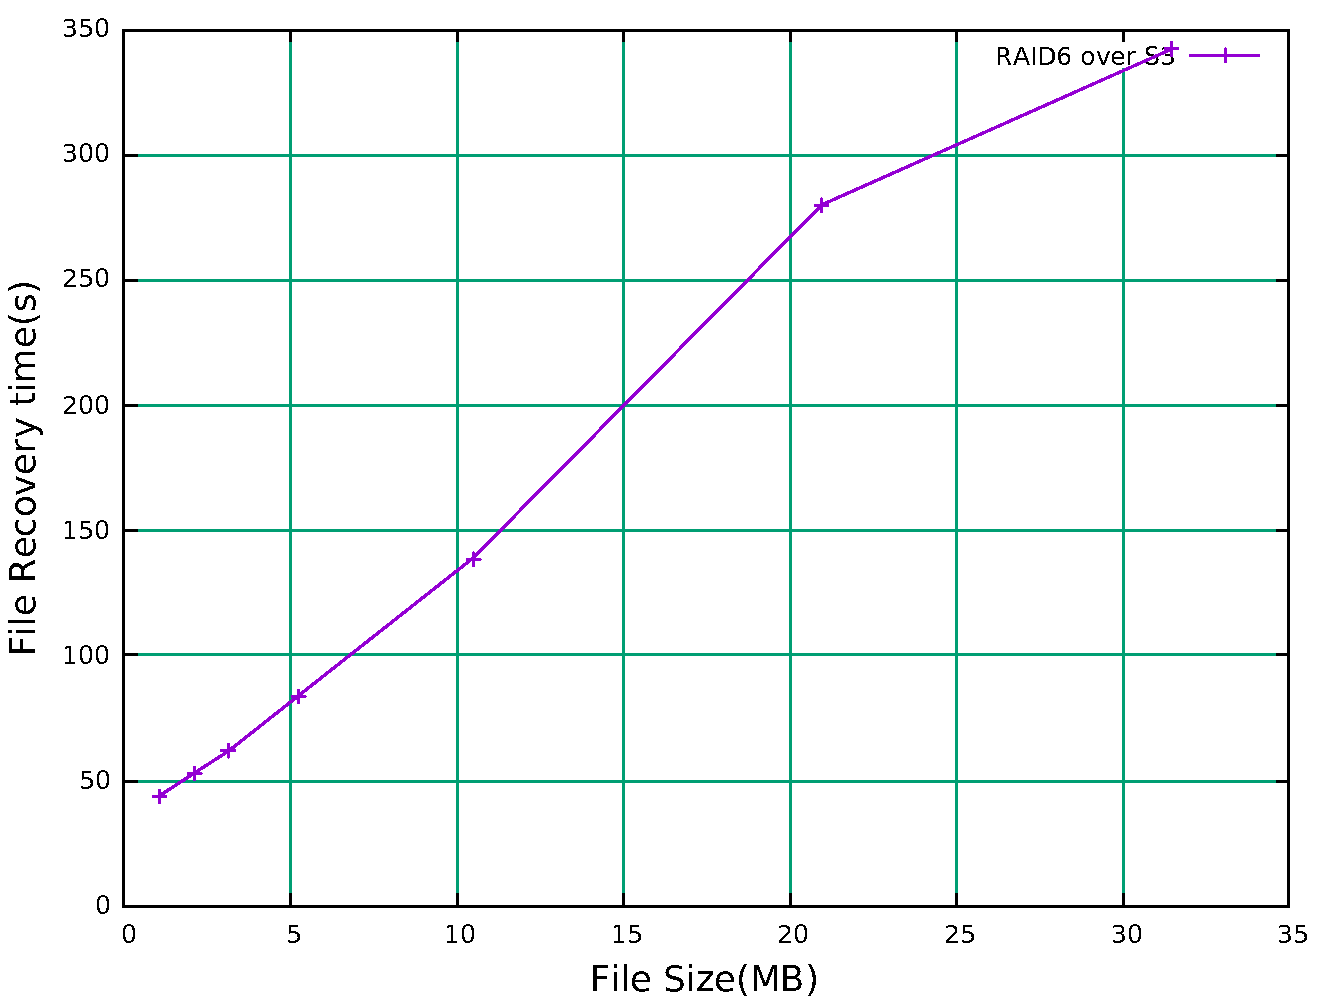
\includegraphics[width=\linewidth]{figures/S3RAIDRecoveryTime.pdf}
\centering
\caption{The Recovery time in seconds of $M=2$ deleted buckets(disks) for varying file sizes.}
\label{fig:S3R6Rcv}
\end{figure}

Afterwards, we quantity the effect of varying chunk size on file store and disk recover time.
To be thorough, we repeat the following experiment for 2 files of size 1MB and 5MB.
For each file we change the chunk size of the S3-RAID6 array varying from $8, 16, 32, 64, 128, 256$. For each file of 1MB and 5MB, we estimate the variation of file save time in Fig.\ref{fig:S3R6StrCHK1MB} and Fig.\ref{fig:S3R6StrCHK5MB}.
Afterwards, we then delete a single bucket from the S3-RAID6 array and compute the recovery time for each chunk.
We present this result in Fig.\ref{fig:S3R6RcvCHK1MB} and Fig.\ref{fig:S3R6RcvCHK5MB}. 

\begin{figure}[h]
\centering
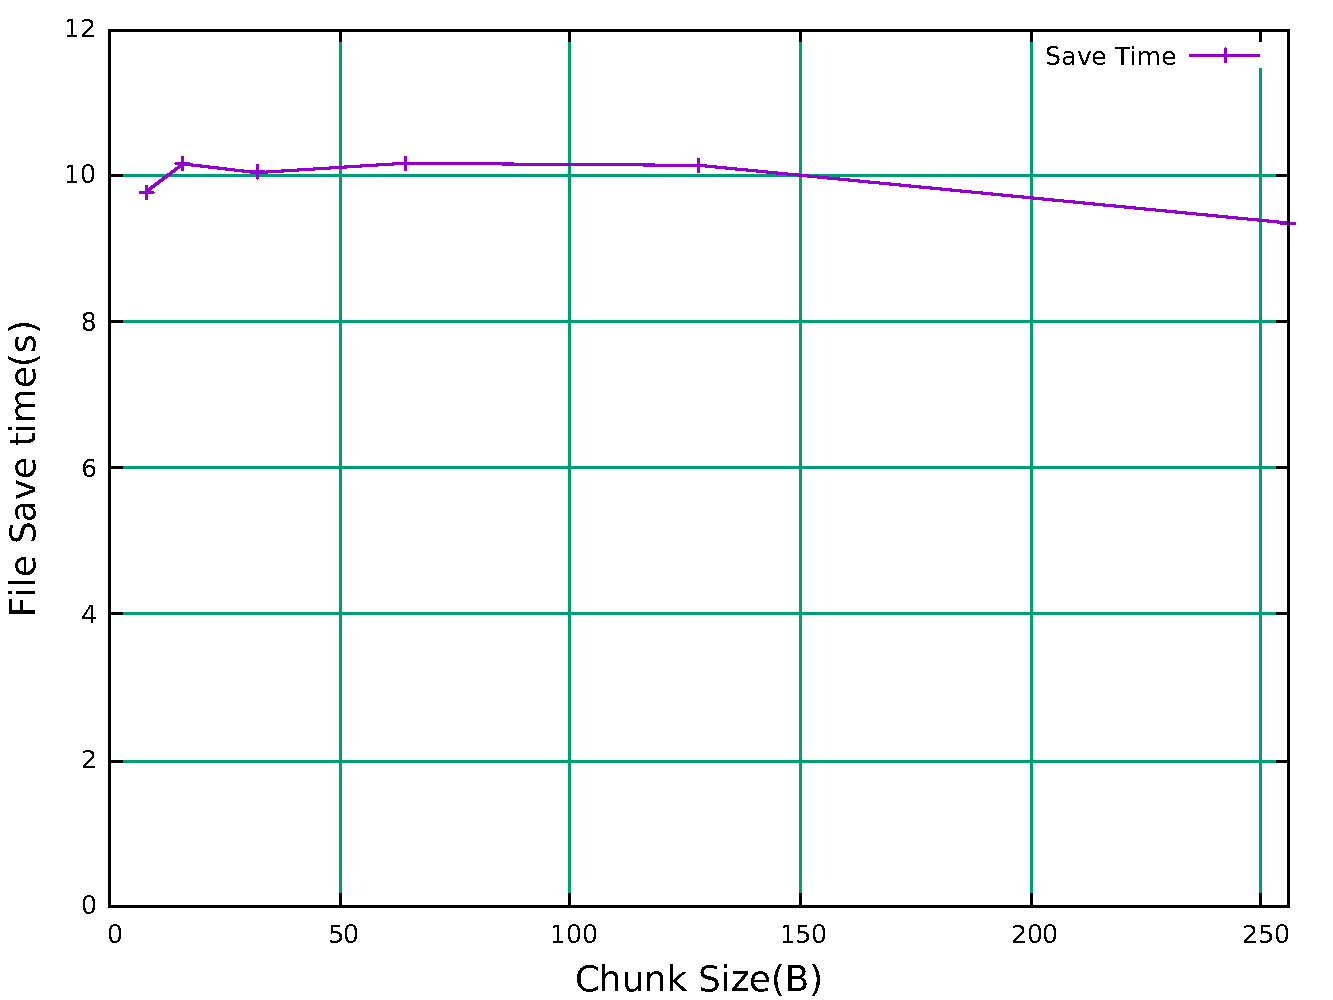
\includegraphics[width=\linewidth]{figures/RAIDStoreTimeChuckSize1Mb.pdf}
\caption{Time duration in seconds to store a file in S3 for varying Chunk sizes under a fixed file size of 1MB}
\label{fig:S3R6StrCHK1MB}
\end{figure}

\begin{figure}[h]
\centering
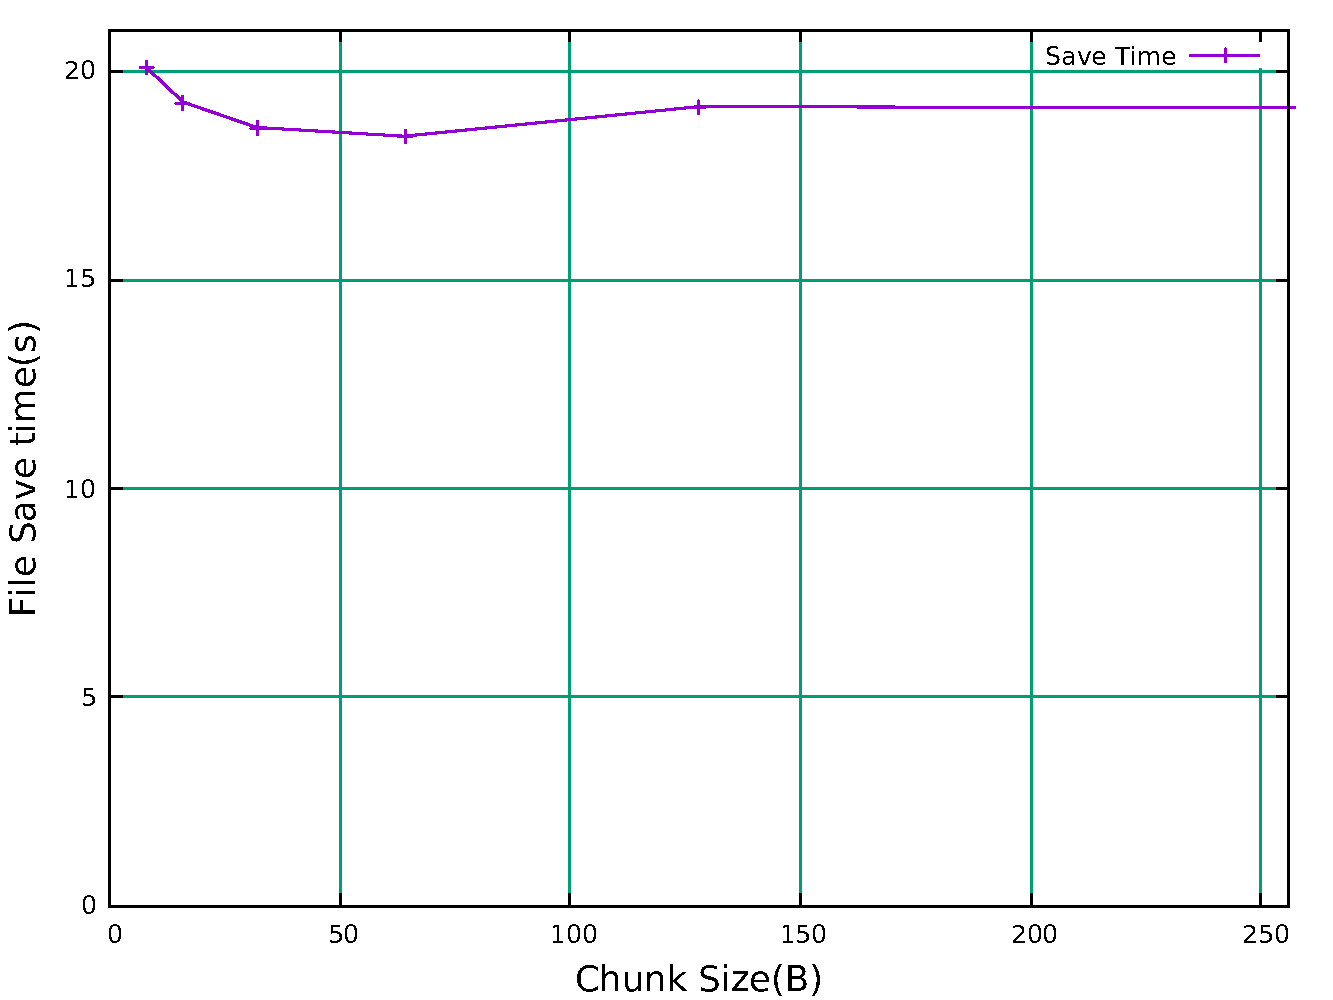
\includegraphics[width=\linewidth]{figures/RAIDStoreTimeChuckSize5Mb.pdf}
\caption{Time duration in seconds to store a file in S3 for varying Chunk sizes under a fixed file size of 5MB}
\label{fig:S3R6StrCHK5MB}
\end{figure}

\begin{figure}[h]
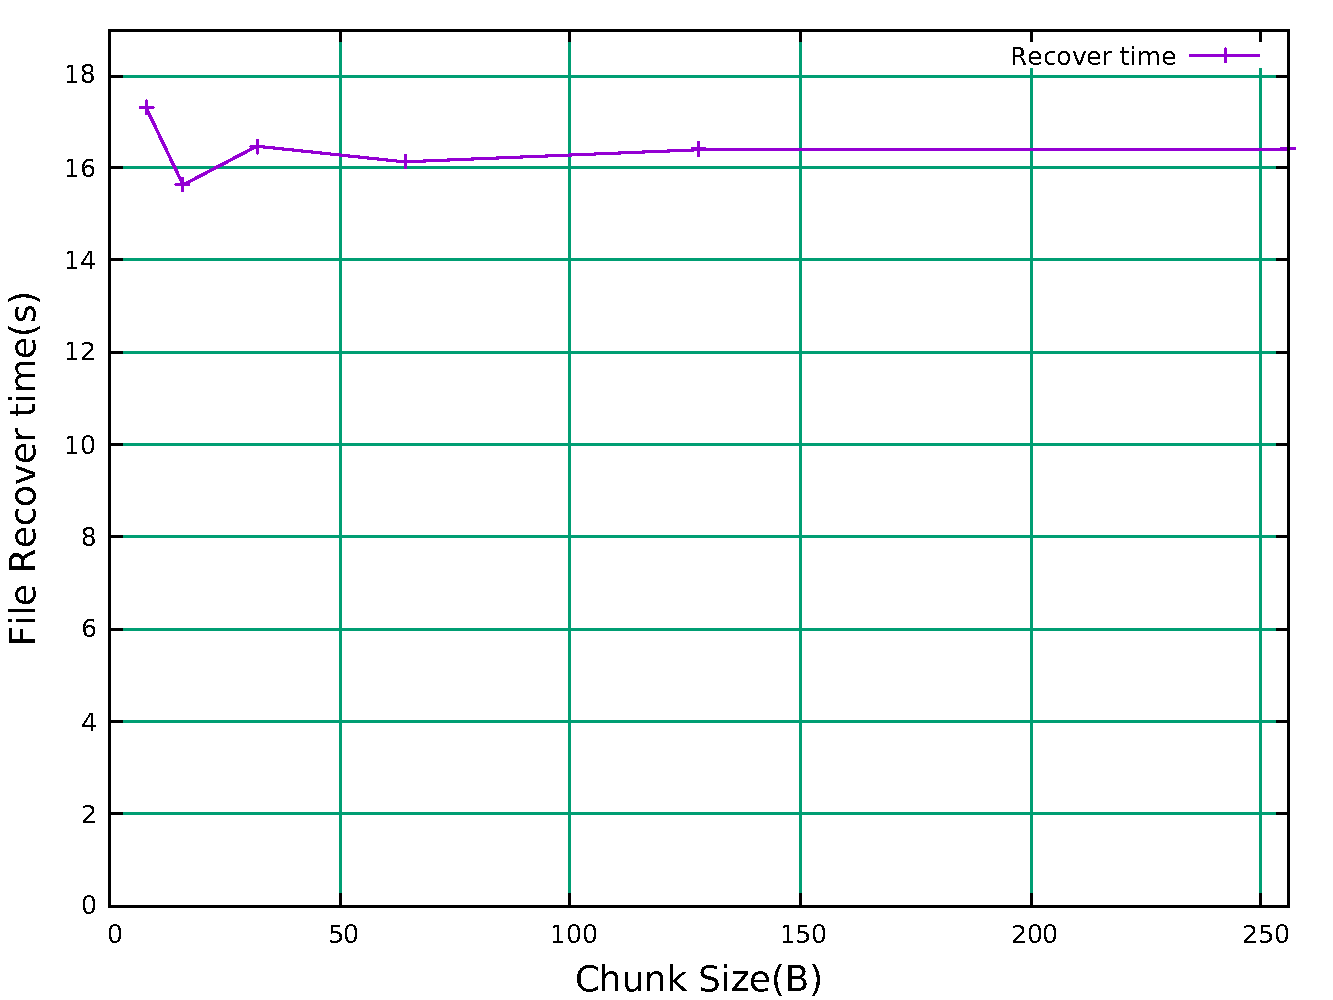
\includegraphics[width=\linewidth]{figures/RAIDRecoverTimeChuckSize1Mb.pdf}
\centering
\caption{Disk Recover time in seconds for varying Chunk sizes under a fixed file size of 1MB}
\label{fig:S3R6RcvCHK1MB}
\end{figure}

\begin{figure}[h]
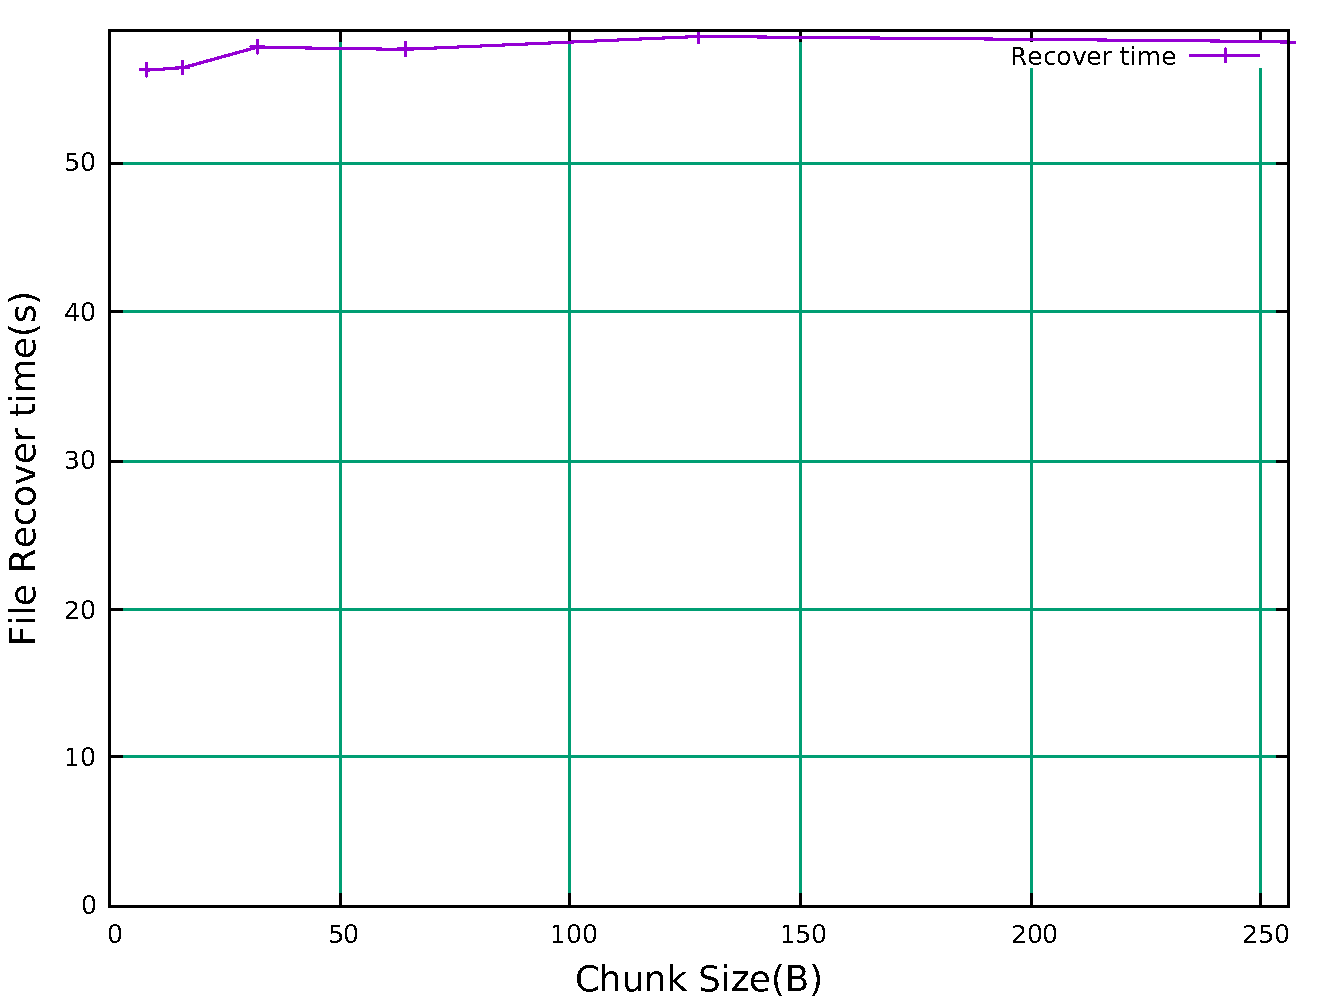
\includegraphics[width=\linewidth]{figures/RAIDRecoverTimeChuckSize5Mb.pdf}
\centering
\caption{Disk Recover time in seconds for varying Chunk sizes under a fixed file size of 5MB}
\label{fig:S3R6RcvCHK5MB}
\end{figure}
